\begin{figure}
\begin{tabular}{@{}c@{}c@{}}
\begin{subfigure}[b]{0.4\textwidth}
\begin{center}
\begin{spacing}{1.5}
\begin{allLangEnvScript}
~{\scriptsize \textcolor{mygray}{D0:}}~ List ${\tt Clist_{\mem{}}^{lnode}}$(i32 l) {
~{\scriptsize \textcolor{mygray}{D1:}}~  if l = 0:
~{\scriptsize \textcolor{mygray}{D2:}}~   return LNil;
~{\scriptsize \textcolor{mygray}{D3:}}~  else:
~{\scriptsize \textcolor{mygray}{D4:}}~   i32  val  $\coloneqq$ $\structPointer{l}{\mem{}}{lnode}{val}$;
~{\scriptsize \textcolor{mygray}{D5:}}~   List tail $\coloneqq$ ${\tt Clist_{\mem{}}^{lnode}}$($\structPointer{l}{\mem{}}{lnode}{next}$);
~{\scriptsize \textcolor{mygray}{D6:}}~   return LCons(val, tail);
~{\scriptsize \textcolor{mygray}{DE:}}~ }
\end{allLangEnvScript}
\end{spacing}
\end{center}
\vspace{8px}
\caption{\label{fig:clistdeconsIR}(Abstracted) IR of Deconstruction Program}
\end{subfigure}%
&
\begin{subfigure}[b]{0.6\textwidth}
\begin{center}
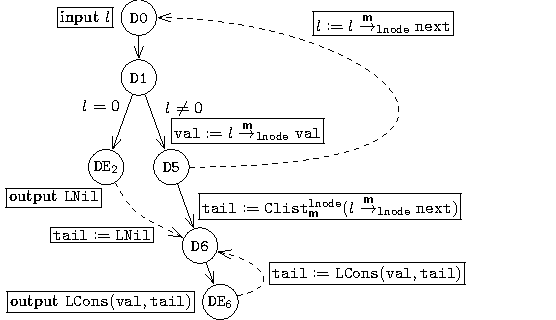
\includegraphics[scale=1]{chapters/figures/figClistDeconsCfg.pdf}
\end{center}
\vspace{5px}
\caption{\label{fig:clistdeconsCFG}CFG of Deconstruction Program}
\end{subfigure}%
\\
\end{tabular}
\caption{\label{fig:clistdecons}IR and CFG representation of deconstruction program based on the lifting constructor \lift{list}{}{lnode} defined in \cref{eqn:clist}.
In \cref{fig:clistdeconsIR}, \dpc{6} contains a recursive function call. In \cref{fig:clistdeconsCFG}, the square boxes show the transfer functions for the deconstruction program.
The dashed edges represent the recursive function call in the CFG representation as shown in \cref{fig:clistdeconsCFG}.}
\end{figure}